\documentclass[12pt,a4paper]{article}
\usepackage[utf8]{vietnam}
\usepackage{amsmath,amssymb}
\usepackage{tabularx}
\usepackage{tikz}
\usepackage{xcolor}
\usepackage[top=0.6cm, bottom=0.6cm, left=0.6cm, right=0.6cm]{geometry}
\usepackage[dethi]{ex_test}

\SAOPTN{widthSA=2.6,heightSA=0.62}
\setlength{\parskip}{0pt}

% Dong ke cham mo chuan viet tay
\newcommand{\dongke}[1]{%
  \begingroup%
  \setlength{\parskip}{0pt}%
  \baselineskip=18.5pt%
  \vspace{1.0mm}%
  \foreach \i in {1,...,#1}{%
    \noindent{\color{gray!60}\dotfill}\par%
  }%
  \vspace{0.6mm}%
  \endgroup%
}

% Khu vuc bai lam chia 2 cot co vach ngan mo o giua
\newcommand{\dongkeHaiCot}[1]{%
  \par\vspace{0.5mm}%
  \noindent%
  \begin{minipage}[t]{0.485\linewidth}%
    \dongke{#1}%
  \end{minipage}%
  \hfill%
  {\color{gray!60}\vrule}%
  \hfill%
  \begin{minipage}[t]{0.485\linewidth}%
    \dongke{#1}%
  \end{minipage}%
}

% Dinh nghia o bai tap tu luan trong bang
\newcommand{\oBaiTap}[3][5]{%
  \vspace{1.0mm}%
  \noindent\textbf{#2} #3\par%
  \dongke{#1}%
}

\begin{document}
\pagestyle{empty}
% =============================================================================
% ========================= TOAN 7 TUAN 10 BUOI 02 - MA DE 101 =================
% ========================= TRANG 1/2 ==========================================
% =============================================================================
\noindent
\begin{tabularx}{\linewidth}{|X|c|}
\hline
\textbf{PHIẾU KIỂM TRA ĐỊNH KỲ TOÁN 7 - TUẦN 10 - BUỔI 2} & \textbf{Mã đề: 101 - Trang 1/2} \\
\hline
\end{tabularx}

\vspace{1.2mm}

\noindent
\begin{tabularx}{\linewidth}{|p{3.2cm}|X|}
\hline
\centering\textbf{ĐIỂM SỐ} & \centering\textbf{LỜI NHẬN XÉT CỦA THẦY CÔ} \tabularnewline
\hline
\rule{0pt}{1.8cm} & \tabularnewline
\hline
\end{tabularx}

\vspace{1.5mm}
\noindent\textbf{Câu 1 (0,25 điểm).} Số đối của số hữu tỉ $\dfrac{4}{9}$ là: \shortans{-\dfrac{4}{9}}\par\vspace{1.8mm}
\noindent\textbf{Câu 2 (0,25 điểm).} Giá trị của $\sqrt{144}$ là: \shortans{12}\par\vspace{1.8mm}
\noindent\textbf{Câu 3 (0,25 điểm).} Giá trị tuyệt đối $|-7{,}82| = $ \shortans{7{,}82}\par\vspace{1.8mm}
\noindent\textbf{Câu 4 (0,25 điểm).} Ba cạnh $\Delta$ này bằng ba cạnh $\Delta$ kia thì hai $\Delta$ đó: \shortans{\text{bằng nhau}}\par\vspace{1.8mm}
\noindent\textbf{Câu 5 (0,25 điểm).} Cho $\Delta ABC = \Delta CDA, \widehat{BAC}=35^\circ$. Số đo góc $\widehat{DCA}$ là: \shortans{35^\circ}\par\vspace{1.8mm}
\noindent\textbf{Câu 6 (0,25 điểm).} Có $\widehat{BAC} = \widehat{DCA}$ so le trong suy ra hai đường thẳng: \shortans{AB \parallel CD}\par\vspace{1.8mm}
\noindent\textbf{Câu 7 (0,25 điểm).} Cho $\Delta ABM = \Delta ACM$, $\widehat{AMB}$ và $\widehat{AMC}$ kề bù thì $\widehat{AMB} = $ \shortans{90^\circ}\par\vspace{1.8mm}
\noindent\textbf{Câu 8 (0,25 điểm).} Tứ giác $ABCD$ ($AB=CD, BC=DA$). Cạnh chung $\Delta ABC, \Delta CDA$ là: \shortans{AC}\par\vspace{1.8mm}
\noindent\textbf{Câu 9 (0,25 điểm).} Dùng compa vẽ 2 cung tròn cắt nhau tại $C$, tia $OC$ là: \shortans{\text{phân giác}}\par\vspace{1.8mm}
\noindent\textbf{Câu 10 (0,25 điểm).} Cổng sắt có thanh giằng chéo không xệ nhờ tính cứng vững của: \shortans{\text{tam giác}}\par\vspace{1.8mm}
\vspace{0.2mm}
\noindent\textbf{Câu 11 (3,0 điểm). Thực hiện phép tính (hợp lý nếu có thể):}
\vspace{0.8mm}

\noindent
\begin{tabularx}{\linewidth}{|X|X|}
\hline
\oBaiTap[5]{a) (0,5 điểm)}{\dfrac{7}{10} + \dfrac{11}{20} - \dfrac{1}{4}} & 
\oBaiTap[5]{b) (0,5 điểm)}{\dfrac{7}{15} \cdot \left(-\dfrac{5}{8}\right) + \dfrac{7}{15} \cdot \left(-\dfrac{3}{8}\right)} \\
\hline
\oBaiTap[5]{c) (0,5 điểm)}{\left(-\dfrac{1}{3}\right)^3 \cdot 27 + \dfrac{4}{9} : \dfrac{2}{9}} & 
\oBaiTap[5]{d) (0,5 điểm)}{\sqrt{\dfrac{100}{49}} - \left|-\dfrac{4}{7}\right| + \dfrac{1}{7}} \\
\hline
\oBaiTap[5]{e) (0,5 điểm)}{\dfrac{10}{3} - \left[\dfrac{4}{3} + \left(\dfrac{1}{2}\right)^3 \cdot 8\right]} & 
\oBaiTap[5]{f) (0,5 điểm)}{\dfrac{3^{10} \cdot 8^3}{2^8 \cdot 9^4}} \\
\hline
\end{tabularx}

\newpage
% =============================================================================
% ========================= TOAN 7 TUAN 10 BUOI 02 - MA DE 101 =================
% ========================= TRANG 2/2 ==========================================
% =============================================================================
\noindent
\begin{tabularx}{\linewidth}{|X|c|}
\hline
\textbf{TOÁN 7 - TUẦN 10 - BUỔI 2} & \textbf{Mã đề: 101 - Trang 2/2} \\
\hline
\end{tabularx}

\vspace{1.5mm}

\noindent\textbf{Câu 12 (2,0 điểm). Tìm số hữu tỉ $x$, biết:}
\vspace{0.8mm}

\noindent
\begin{tabularx}{\linewidth}{|X|X|}
\hline
\oBaiTap[5]{a) (0,5 điểm)}{x + \dfrac{3}{7} = \dfrac{11}{14}} & 
\oBaiTap[5]{b) (0,5 điểm)}{\dfrac{5}{6} - \dfrac{2}{3}x = \dfrac{1}{2}} \\
\hline
\oBaiTap[5]{c) (0,5 điểm)}{\left(2x - \dfrac{1}{3}\right)^2 = \dfrac{25}{9}} & 
\oBaiTap[5]{d) (0,5 điểm)}{\left|3x + \dfrac{1}{2}\right| = \dfrac{7}{2}} \\
\hline
\end{tabularx}

\vspace{1.5mm}

\noindent
\begin{tabularx}{\linewidth}{|X|}
\hline
\vspace{0.5mm}
\begin{minipage}[t]{0.68\linewidth}
\vspace{0pt}
\textbf{Câu 13 (2,0 điểm).} Cho tứ giác $ABCD$ có $AB = CD$ và $BC = DA$. Nối hai đỉnh $A$ và $C$.\par\vspace{0.4mm}
\textbf{a)} (1,0 điểm) Chứng minh rằng $\Delta ABC = \Delta CDA$.\par\vspace{0.4mm}
\textbf{b)} (1,0 điểm) Chứng minh $AB \parallel CD$ và $AD \parallel BC$. Biết $\widehat{B} = 110^\circ, \widehat{BAC} = 30^\circ$, tính số đo các góc $\widehat{D}$ và $\widehat{DCA}$.
\end{minipage}\hfill
\begin{minipage}[t]{0.30\linewidth}
\vspace{0pt}\centering
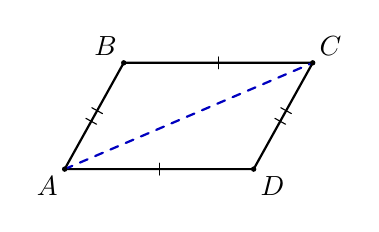
\begin{tikzpicture}[scale=0.75, >=stealth, line join=round, line cap=round]
  \coordinate (A) at (0, 0);
  \coordinate (D) at (3.2, 0);
  \coordinate (B) at (1.0, 1.8);
  \coordinate (C) at (4.2, 1.8);
  
  % Canh tu giac
  \draw[thick] (A) -- (B) -- (C) -- (D) -- cycle;
  % Duong cheo AC
  \draw[thick, dashed, blue!75!black] (A) -- (C);
  
  % Vach danh dau AB = CD (2 vach cat ngang)
  \draw (0.45 - 0.09, 0.81 + 0.05) -- (0.45 + 0.09, 0.81 - 0.05);
  \draw (0.55 - 0.09, 0.99 + 0.05) -- (0.55 + 0.09, 0.99 - 0.05);
  \draw (3.65 - 0.09, 0.81 + 0.05) -- (3.65 + 0.09, 0.81 - 0.05);
  \draw (3.75 - 0.09, 0.99 + 0.05) -- (3.75 + 0.09, 0.99 - 0.05);
  
  % Vach danh dau AD = BC (1 vach cat ngang)
  \draw (1.6, -0.1) -- (1.6, 0.1);
  \draw (2.6, 1.7) -- (2.6, 1.9);
  
  % Cac diem
  \fill (A) circle (1.3pt) node[below left=-1pt] {$A$};
  \fill (B) circle (1.3pt) node[above left=-1pt] {$B$};
  \fill (C) circle (1.3pt) node[above right=-1pt] {$C$};
  \fill (D) circle (1.3pt) node[below right=-1pt] {$D$};
\end{tikzpicture}
\end{minipage}\par
\vspace{0.4mm}
\noindent\textit{Bài giải:}\dongkeHaiCot{11}
\\ \hline
\end{tabularx}

\vspace{1.5mm}

\noindent
\begin{tabularx}{\linewidth}{|X|}
\hline
\vspace{0.5mm}
\textbf{Câu 14 (0,5 điểm).} Tìm giá trị lớn nhất của biểu thức: $B = \dfrac{12}{|x - 2026| + 3}$.\par
\vspace{0.4mm}
\noindent\textit{Bài giải:}\dongkeHaiCot{6}
\\ \hline
\end{tabularx}

\newpage
% =============================================================================
% ========================= TOAN 7 TUAN 10 BUOI 02 - MA DE 102 =================
% ========================= TRANG 1/2 ==========================================
% =============================================================================
\noindent
\begin{tabularx}{\linewidth}{|X|c|}
\hline
\textbf{PHIẾU KIỂM TRA ĐỊNH KỲ TOÁN 7 - TUẦN 10 - BUỔI 2} & \textbf{Mã đề: 102 - Trang 1/2} \\
\hline
\end{tabularx}

\vspace{1.2mm}

\noindent
\begin{tabularx}{\linewidth}{|p{3.2cm}|X|}
\hline
\centering\textbf{ĐIỂM SỐ} & \centering\textbf{LỜI NHẬN XÉT CỦA THẦY CÔ} \tabularnewline
\hline
\rule{0pt}{1.8cm} & \tabularnewline
\hline
\end{tabularx}

\vspace{1.5mm}
\noindent\textbf{Câu 1 (0,25 điểm).} Số đối của số hữu tỉ $\dfrac{5}{7}$ là: \shortans{-\dfrac{5}{7}}\par\vspace{1.8mm}
\noindent\textbf{Câu 2 (0,25 điểm).} Giá trị của $\sqrt{169}$ là: \shortans{13}\par\vspace{1.8mm}
\noindent\textbf{Câu 3 (0,25 điểm).} Giá trị tuyệt đối $|-4{,}95| = $ \shortans{4{,}95}\par\vspace{1.8mm}
\noindent\textbf{Câu 4 (0,25 điểm).} Ba cạnh $\Delta$ này bằng ba cạnh $\Delta$ kia thì hai $\Delta$ đó: \shortans{\text{bằng nhau}}\par\vspace{1.8mm}
\noindent\textbf{Câu 5 (0,25 điểm).} Cho $\Delta ABC = \Delta CDA, \widehat{BCA}=42^\circ$. Số đo góc $\widehat{DAC}$ là: \shortans{42^\circ}\par\vspace{1.8mm}
\noindent\textbf{Câu 6 (0,25 điểm).} Có $\widehat{BCA} = \widehat{DAC}$ so le trong suy ra hai đường thẳng: \shortans{AD \parallel BC}\par\vspace{1.8mm}
\noindent\textbf{Câu 7 (0,25 điểm).} Cho $\Delta HIK = \Delta HIN$, $\widehat{HIK}$ và $\widehat{HIN}$ kề bù thì $\widehat{HIK} = $ \shortans{90^\circ}\par\vspace{1.8mm}
\noindent\textbf{Câu 8 (0,25 điểm).} Tứ giác $MNPQ$ ($MN=PQ, NP=QM$). Cạnh chung $\Delta MNP, \Delta PQM$ là: \shortans{MP}\par\vspace{1.8mm}
\noindent\textbf{Câu 9 (0,25 điểm).} Vẽ $\Delta$ biết độ dài 3 cạnh dựa trên trường hợp bằng nhau: \shortans{\text{c.c.c}}\par\vspace{1.8mm}
\noindent\textbf{Câu 10 (0,25 điểm).} Tháp truyền hình được cấu tạo bởi các thanh kim loại ghép thành: \shortans{\text{hình tam giác}}\par\vspace{1.8mm}
\vspace{0.2mm}
\noindent\textbf{Câu 11 (3,0 điểm). Thực hiện phép tính (hợp lý nếu có thể):}
\vspace{0.8mm}

\noindent
\begin{tabularx}{\linewidth}{|X|X|}
\hline
\oBaiTap[5]{a) (0,5 điểm)}{\dfrac{5}{8} + \dfrac{11}{16} - \dfrac{5}{16}} & 
\oBaiTap[5]{b) (0,5 điểm)}{\dfrac{8}{17} \cdot \left(-\dfrac{7}{12}\right) + \dfrac{8}{17} \cdot \left(-\dfrac{5}{12}\right)} \\
\hline
\oBaiTap[5]{c) (0,5 điểm)}{\left(-\dfrac{1}{2}\right)^4 \cdot 16 + \dfrac{5}{8} : \dfrac{5}{16}} & 
\oBaiTap[5]{d) (0,5 điểm)}{\sqrt{\dfrac{121}{64}} - \left|-\dfrac{5}{8}\right| + \dfrac{2}{8}} \\
\hline
\oBaiTap[5]{e) (0,5 điểm)}{\dfrac{11}{3} - \left[\dfrac{5}{3} + \left(\dfrac{1}{3}\right)^2 \cdot 9\right]} & 
\oBaiTap[5]{f) (0,5 điểm)}{\dfrac{2^{11} \cdot 27^3}{3^8 \cdot 4^5}} \\
\hline
\end{tabularx}

\newpage
% =============================================================================
% ========================= TOAN 7 TUAN 10 BUOI 02 - MA DE 102 =================
% ========================= TRANG 2/2 ==========================================
% =============================================================================
\noindent
\begin{tabularx}{\linewidth}{|X|c|}
\hline
\textbf{TOÁN 7 - TUẦN 10 - BUỔI 2} & \textbf{Mã đề: 102 - Trang 2/2} \\
\hline
\end{tabularx}

\vspace{1.5mm}

\noindent\textbf{Câu 12 (2,0 điểm). Tìm số hữu tỉ $x$, biết:}
\vspace{0.8mm}

\noindent
\begin{tabularx}{\linewidth}{|X|X|}
\hline
\oBaiTap[5]{a) (0,5 điểm)}{x + \dfrac{2}{5} = \dfrac{9}{10}} & 
\oBaiTap[5]{b) (0,5 điểm)}{\dfrac{7}{8} - \dfrac{3}{4}x = \dfrac{1}{8}} \\
\hline
\oBaiTap[5]{c) (0,5 điểm)}{\left(2x - \dfrac{1}{2}\right)^2 = \dfrac{9}{4}} & 
\oBaiTap[5]{d) (0,5 điểm)}{\left|2x + \dfrac{1}{3}\right| = \dfrac{7}{3}} \\
\hline
\end{tabularx}

\vspace{1.5mm}

\noindent
\begin{tabularx}{\linewidth}{|X|}
\hline
\vspace{0.5mm}
\begin{minipage}[t]{0.68\linewidth}
\vspace{0pt}
\textbf{Câu 13 (2,0 điểm).} Cho tứ giác $ABCD$ có $AB = CD$ và $BC = DA$. Nối hai đỉnh $A$ và $C$.\par\vspace{0.4mm}
\textbf{a)} (1,0 điểm) Chứng minh rằng $\Delta ABC = \Delta CDA$.\par\vspace{0.4mm}
\textbf{b)} (1,0 điểm) Chứng minh $AB \parallel CD$ và $AD \parallel BC$. Biết $\widehat{B} = 115^\circ, \widehat{BAC} = 25^\circ$, tính số đo các góc $\widehat{D}$ và $\widehat{DCA}$.
\end{minipage}\hfill
\begin{minipage}[t]{0.30\linewidth}
\vspace{0pt}\centering
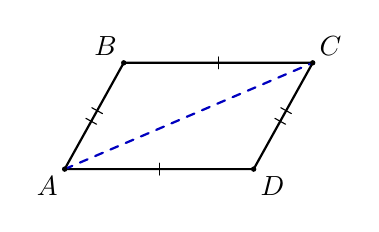
\begin{tikzpicture}[scale=0.75, >=stealth, line join=round, line cap=round]
  \coordinate (A) at (0, 0);
  \coordinate (D) at (3.2, 0);
  \coordinate (B) at (1.0, 1.8);
  \coordinate (C) at (4.2, 1.8);
  
  % Canh tu giac
  \draw[thick] (A) -- (B) -- (C) -- (D) -- cycle;
  % Duong cheo AC
  \draw[thick, dashed, blue!75!black] (A) -- (C);
  
  % Vach danh dau AB = CD (2 vach cat ngang)
  \draw (0.45 - 0.09, 0.81 + 0.05) -- (0.45 + 0.09, 0.81 - 0.05);
  \draw (0.55 - 0.09, 0.99 + 0.05) -- (0.55 + 0.09, 0.99 - 0.05);
  \draw (3.65 - 0.09, 0.81 + 0.05) -- (3.65 + 0.09, 0.81 - 0.05);
  \draw (3.75 - 0.09, 0.99 + 0.05) -- (3.75 + 0.09, 0.99 - 0.05);
  
  % Vach danh dau AD = BC (1 vach cat ngang)
  \draw (1.6, -0.1) -- (1.6, 0.1);
  \draw (2.6, 1.7) -- (2.6, 1.9);
  
  % Cac diem
  \fill (A) circle (1.3pt) node[below left=-1pt] {$A$};
  \fill (B) circle (1.3pt) node[above left=-1pt] {$B$};
  \fill (C) circle (1.3pt) node[above right=-1pt] {$C$};
  \fill (D) circle (1.3pt) node[below right=-1pt] {$D$};
\end{tikzpicture}
\end{minipage}\par
\vspace{0.4mm}
\noindent\textit{Bài giải:}\dongkeHaiCot{11}
\\ \hline
\end{tabularx}

\vspace{1.5mm}

\noindent
\begin{tabularx}{\linewidth}{|X|}
\hline
\vspace{0.5mm}
\textbf{Câu 14 (0,5 điểm).} Tìm giá trị lớn nhất của biểu thức: $B = \dfrac{15}{|x - 2025| + 5}$.\par
\vspace{0.4mm}
\noindent\textit{Bài giải:}\dongkeHaiCot{6}
\\ \hline
\end{tabularx}

\newpage
% =============================================================================
% ========================= TOAN 7 TUAN 10 BUOI 02 - MA DE 103 =================
% ========================= TRANG 1/2 ==========================================
% =============================================================================
\noindent
\begin{tabularx}{\linewidth}{|X|c|}
\hline
\textbf{PHIẾU KIỂM TRA ĐỊNH KỲ TOÁN 7 - TUẦN 10 - BUỔI 2} & \textbf{Mã đề: 103 - Trang 1/2} \\
\hline
\end{tabularx}

\vspace{1.2mm}

\noindent
\begin{tabularx}{\linewidth}{|p{3.2cm}|X|}
\hline
\centering\textbf{ĐIỂM SỐ} & \centering\textbf{LỜI NHẬN XÉT CỦA THẦY CÔ} \tabularnewline
\hline
\rule{0pt}{1.8cm} & \tabularnewline
\hline
\end{tabularx}

\vspace{1.5mm}
\noindent\textbf{Câu 1 (0,25 điểm).} Số đối của số hữu tỉ $\dfrac{3}{11}$ là: \shortans{-\dfrac{3}{11}}\par\vspace{1.8mm}
\noindent\textbf{Câu 2 (0,25 điểm).} Giá trị của $\sqrt{196}$ là: \shortans{14}\par\vspace{1.8mm}
\noindent\textbf{Câu 3 (0,25 điểm).} Giá trị tuyệt đối $|-6{,}38| = $ \shortans{6{,}38}\par\vspace{1.8mm}
\noindent\textbf{Câu 4 (0,25 điểm).} Ba cạnh $\Delta$ này bằng ba cạnh $\Delta$ kia thì hai $\Delta$ đó: \shortans{\text{bằng nhau}}\par\vspace{1.8mm}
\noindent\textbf{Câu 5 (0,25 điểm).} Cho $\Delta MNP = \Delta QPN, \widehat{MNP}=48^\circ$. Số đo góc $\widehat{QPN}$ là: \shortans{48^\circ}\par\vspace{1.8mm}
\noindent\textbf{Câu 6 (0,25 điểm).} Có $\widehat{MNP} = \widehat{QPN}$ so le trong suy ra hai đường thẳng: \shortans{MN \parallel PQ}\par\vspace{1.8mm}
\noindent\textbf{Câu 7 (0,25 điểm).} Cho $\Delta DEF = \Delta DEG$, $\widehat{DEF}$ và $\widehat{DEG}$ kề bù thì $\widehat{DEF} = $ \shortans{90^\circ}\par\vspace{1.8mm}
\noindent\textbf{Câu 8 (0,25 điểm).} Tứ giác $ABCD$ ($AB=AD, CB=CD$). Cạnh chung $\Delta ABC, \Delta ADC$ là: \shortans{AC}\par\vspace{1.8mm}
\noindent\textbf{Câu 9 (0,25 điểm).} Để kiểm tra 2 tam giác bằng gỗ có bằng nhau, chỉ cần đo: \shortans{\text{3 cạnh}}\par\vspace{1.8mm}
\noindent\textbf{Câu 10 (0,25 điểm).} Khung xe đạp thể thao cấu tạo gồm các hình tam giác giúp xe: \shortans{\text{cứng vững}}\par\vspace{1.8mm}
\vspace{0.2mm}
\noindent\textbf{Câu 11 (3,0 điểm). Thực hiện phép tính (hợp lý nếu có thể):}
\vspace{0.8mm}

\noindent
\begin{tabularx}{\linewidth}{|X|X|}
\hline
\oBaiTap[5]{a) (0,5 điểm)}{\dfrac{4}{9} + \dfrac{13}{18} - \dfrac{1}{6}} & 
\oBaiTap[5]{b) (0,5 điểm)}{\dfrac{9}{19} \cdot \left(-\dfrac{8}{13}\right) + \dfrac{9}{19} \cdot \left(-\dfrac{5}{13}\right)} \\
\hline
\oBaiTap[5]{c) (0,5 điểm)}{\left(-\dfrac{1}{5}\right)^2 \cdot 25 + \dfrac{6}{7} : \dfrac{3}{7}} & 
\oBaiTap[5]{d) (0,5 điểm)}{\sqrt{\dfrac{144}{81}} - \left|-\dfrac{5}{9}\right| + \dfrac{2}{9}} \\
\hline
\oBaiTap[5]{e) (0,5 điểm)}{\dfrac{13}{4} - \left[\dfrac{5}{4} + \left(\dfrac{1}{2}\right)^2 \cdot 4\right]} & 
\oBaiTap[5]{f) (0,5 điểm)}{\dfrac{5^{10} \cdot 6^4}{15^4 \cdot 25^2}} \\
\hline
\end{tabularx}

\newpage
% =============================================================================
% ========================= TOAN 7 TUAN 10 BUOI 02 - MA DE 103 =================
% ========================= TRANG 2/2 ==========================================
% =============================================================================
\noindent
\begin{tabularx}{\linewidth}{|X|c|}
\hline
\textbf{TOÁN 7 - TUẦN 10 - BUỔI 2} & \textbf{Mã đề: 103 - Trang 2/2} \\
\hline
\end{tabularx}

\vspace{1.5mm}

\noindent\textbf{Câu 12 (2,0 điểm). Tìm số hữu tỉ $x$, biết:}
\vspace{0.8mm}

\noindent
\begin{tabularx}{\linewidth}{|X|X|}
\hline
\oBaiTap[5]{a) (0,5 điểm)}{x + \dfrac{3}{8} = \dfrac{11}{16}} & 
\oBaiTap[5]{b) (0,5 điểm)}{\dfrac{4}{5} - \dfrac{3}{5}x = \dfrac{1}{5}} \\
\hline
\oBaiTap[5]{c) (0,5 điểm)}{\left(3x - \dfrac{1}{2}\right)^2 = \dfrac{25}{4}} & 
\oBaiTap[5]{d) (0,5 điểm)}{\left|4x + \dfrac{1}{2}\right| = \dfrac{9}{2}} \\
\hline
\end{tabularx}

\vspace{1.5mm}

\noindent
\begin{tabularx}{\linewidth}{|X|}
\hline
\vspace{0.5mm}
\begin{minipage}[t]{0.68\linewidth}
\vspace{0pt}
\textbf{Câu 13 (2,0 điểm).} Cho tứ giác $ABCD$ có $AB = CD$ và $BC = DA$. Nối hai đỉnh $A$ và $C$.\par\vspace{0.4mm}
\textbf{a)} (1,0 điểm) Chứng minh rằng $\Delta ABC = \Delta CDA$.\par\vspace{0.4mm}
\textbf{b)} (1,0 điểm) Chứng minh $AB \parallel CD$ và $AD \parallel BC$. Biết $\widehat{B} = 105^\circ, \widehat{BAC} = 35^\circ$, tính số đo các góc $\widehat{D}$ và $\widehat{DCA}$.
\end{minipage}\hfill
\begin{minipage}[t]{0.30\linewidth}
\vspace{0pt}\centering
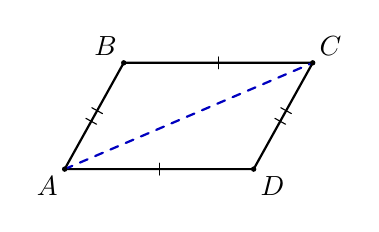
\begin{tikzpicture}[scale=0.75, >=stealth, line join=round, line cap=round]
  \coordinate (A) at (0, 0);
  \coordinate (D) at (3.2, 0);
  \coordinate (B) at (1.0, 1.8);
  \coordinate (C) at (4.2, 1.8);
  
  % Canh tu giac
  \draw[thick] (A) -- (B) -- (C) -- (D) -- cycle;
  % Duong cheo AC
  \draw[thick, dashed, blue!75!black] (A) -- (C);
  
  % Vach danh dau AB = CD (2 vach cat ngang)
  \draw (0.45 - 0.09, 0.81 + 0.05) -- (0.45 + 0.09, 0.81 - 0.05);
  \draw (0.55 - 0.09, 0.99 + 0.05) -- (0.55 + 0.09, 0.99 - 0.05);
  \draw (3.65 - 0.09, 0.81 + 0.05) -- (3.65 + 0.09, 0.81 - 0.05);
  \draw (3.75 - 0.09, 0.99 + 0.05) -- (3.75 + 0.09, 0.99 - 0.05);
  
  % Vach danh dau AD = BC (1 vach cat ngang)
  \draw (1.6, -0.1) -- (1.6, 0.1);
  \draw (2.6, 1.7) -- (2.6, 1.9);
  
  % Cac diem
  \fill (A) circle (1.3pt) node[below left=-1pt] {$A$};
  \fill (B) circle (1.3pt) node[above left=-1pt] {$B$};
  \fill (C) circle (1.3pt) node[above right=-1pt] {$C$};
  \fill (D) circle (1.3pt) node[below right=-1pt] {$D$};
\end{tikzpicture}
\end{minipage}\par
\vspace{0.4mm}
\noindent\textit{Bài giải:}\dongkeHaiCot{11}
\\ \hline
\end{tabularx}

\vspace{1.5mm}

\noindent
\begin{tabularx}{\linewidth}{|X|}
\hline
\vspace{0.5mm}
\textbf{Câu 14 (0,5 điểm).} Tìm giá trị lớn nhất của biểu thức: $B = \dfrac{18}{|x - 2024| + 6}$.\par
\vspace{0.4mm}
\noindent\textit{Bài giải:}\dongkeHaiCot{6}
\\ \hline
\end{tabularx}

\newpage
% =============================================================================
% ========================= TOAN 7 TUAN 10 BUOI 02 - MA DE 104 =================
% ========================= TRANG 1/2 ==========================================
% =============================================================================
\noindent
\begin{tabularx}{\linewidth}{|X|c|}
\hline
\textbf{PHIẾU KIỂM TRA ĐỊNH KỲ TOÁN 7 - TUẦN 10 - BUỔI 2} & \textbf{Mã đề: 104 - Trang 1/2} \\
\hline
\end{tabularx}

\vspace{1.2mm}

\noindent
\begin{tabularx}{\linewidth}{|p{3.2cm}|X|}
\hline
\centering\textbf{ĐIỂM SỐ} & \centering\textbf{LỜI NHẬN XÉT CỦA THẦY CÔ} \tabularnewline
\hline
\rule{0pt}{1.8cm} & \tabularnewline
\hline
\end{tabularx}

\vspace{1.5mm}
\noindent\textbf{Câu 1 (0,25 điểm).} Số đối của số hữu tỉ $\dfrac{6}{13}$ là: \shortans{-\dfrac{6}{13}}\par\vspace{1.8mm}
\noindent\textbf{Câu 2 (0,25 điểm).} Giá trị của $\sqrt{225}$ là: \shortans{15}\par\vspace{1.8mm}
\noindent\textbf{Câu 3 (0,25 điểm).} Giá trị tuyệt đối $|-9{,}15| = $ \shortans{9{,}15}\par\vspace{1.8mm}
\noindent\textbf{Câu 4 (0,25 điểm).} Ba cạnh $\Delta$ này bằng ba cạnh $\Delta$ kia thì hai $\Delta$ đó: \shortans{\text{bằng nhau}}\par\vspace{1.8mm}
\noindent\textbf{Câu 5 (0,25 điểm).} Cho $\Delta MNP = \Delta QPN, \widehat{MPN}=38^\circ$. Số đo góc $\widehat{QNP}$ là: \shortans{38^\circ}\par\vspace{1.8mm}
\noindent\textbf{Câu 6 (0,25 điểm).} Có $\widehat{MPN} = \widehat{QNP}$ so le trong suy ra hai đường thẳng: \shortans{MQ \parallel NP}\par\vspace{1.8mm}
\noindent\textbf{Câu 7 (0,25 điểm).} Cho $\Delta PQR = \Delta PQS$, $\widehat{PQR}$ và $\widehat{PQS}$ kề bù thì $\widehat{PQR} = $ \shortans{90^\circ}\par\vspace{1.8mm}
\noindent\textbf{Câu 8 (0,25 điểm).} Tứ giác $EFGH$ ($EF=EH, GF=GH$). Cạnh chung $\Delta EFG, \Delta EHG$ là: \shortans{EG}\par\vspace{1.8mm}
\noindent\textbf{Câu 9 (0,25 điểm).} Biết độ dài 3 cạnh thì vẽ được duy nhất số hình tam giác là: \shortans{1}\par\vspace{1.8mm}
\noindent\textbf{Câu 10 (0,25 điểm).} Khung giá chữ A treo tranh vẽ đứng vững trên mặt sàn nhờ cấu trúc: \shortans{\text{hình tam giác}}\par\vspace{1.8mm}
\vspace{0.2mm}
\noindent\textbf{Câu 11 (3,0 điểm). Thực hiện phép tính (hợp lý nếu có thể):}
\vspace{0.8mm}

\noindent
\begin{tabularx}{\linewidth}{|X|X|}
\hline
\oBaiTap[5]{a) (0,5 điểm)}{\dfrac{5}{12} + \dfrac{17}{24} - \dfrac{1}{8}} & 
\oBaiTap[5]{b) (0,5 điểm)}{\dfrac{11}{21} \cdot \left(-\dfrac{9}{14}\right) + \dfrac{11}{21} \cdot \left(-\dfrac{5}{14}\right)} \\
\hline
\oBaiTap[5]{c) (0,5 điểm)}{\left(-\dfrac{1}{2}\right)^5 \cdot 32 + \dfrac{8}{9} : \dfrac{4}{9}} & 
\oBaiTap[5]{d) (0,5 điểm)}{\sqrt{\dfrac{169}{100}} - \left|-\dfrac{7}{10}\right| + \dfrac{4}{10}} \\
\hline
\oBaiTap[5]{e) (0,5 điểm)}{\dfrac{15}{4} - \left[\dfrac{7}{4} + \left(\dfrac{1}{4}\right) \cdot 4\right]} & 
\oBaiTap[5]{f) (0,5 điểm)}{\dfrac{2^9 \cdot 125^3}{10^7 \cdot 5}} \\
\hline
\end{tabularx}

\newpage
% =============================================================================
% ========================= TOAN 7 TUAN 10 BUOI 02 - MA DE 104 =================
% ========================= TRANG 2/2 ==========================================
% =============================================================================
\noindent
\begin{tabularx}{\linewidth}{|X|c|}
\hline
\textbf{TOÁN 7 - TUẦN 10 - BUỔI 2} & \textbf{Mã đề: 104 - Trang 2/2} \\
\hline
\end{tabularx}

\vspace{1.5mm}

\noindent\textbf{Câu 12 (2,0 điểm). Tìm số hữu tỉ $x$, biết:}
\vspace{0.8mm}

\noindent
\begin{tabularx}{\linewidth}{|X|X|}
\hline
\oBaiTap[5]{a) (0,5 điểm)}{x + \dfrac{4}{9} = \dfrac{13}{18}} & 
\oBaiTap[5]{b) (0,5 điểm)}{\dfrac{5}{6} - \dfrac{1}{2}x = \dfrac{1}{3}} \\
\hline
\oBaiTap[5]{c) (0,5 điểm)}{\left(3x - \dfrac{1}{3}\right)^2 = \dfrac{16}{9}} & 
\oBaiTap[5]{d) (0,5 điểm)}{\left|2x + \dfrac{3}{4}\right| = \dfrac{7}{4}} \\
\hline
\end{tabularx}

\vspace{1.5mm}

\noindent
\begin{tabularx}{\linewidth}{|X|}
\hline
\vspace{0.5mm}
\begin{minipage}[t]{0.68\linewidth}
\vspace{0pt}
\textbf{Câu 13 (2,0 điểm).} Cho tứ giác $ABCD$ có $AB = CD$ và $BC = DA$. Nối hai đỉnh $A$ và $C$.\par\vspace{0.4mm}
\textbf{a)} (1,0 điểm) Chứng minh rằng $\Delta ABC = \Delta CDA$.\par\vspace{0.4mm}
\textbf{b)} (1,0 điểm) Chứng minh $AB \parallel CD$ và $AD \parallel BC$. Biết $\widehat{B} = 120^\circ, \widehat{BAC} = 20^\circ$, tính số đo các góc $\widehat{D}$ và $\widehat{DCA}$.
\end{minipage}\hfill
\begin{minipage}[t]{0.30\linewidth}
\vspace{0pt}\centering
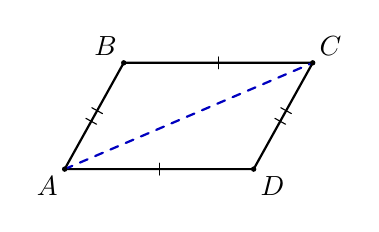
\begin{tikzpicture}[scale=0.75, >=stealth, line join=round, line cap=round]
  \coordinate (A) at (0, 0);
  \coordinate (D) at (3.2, 0);
  \coordinate (B) at (1.0, 1.8);
  \coordinate (C) at (4.2, 1.8);
  
  % Canh tu giac
  \draw[thick] (A) -- (B) -- (C) -- (D) -- cycle;
  % Duong cheo AC
  \draw[thick, dashed, blue!75!black] (A) -- (C);
  
  % Vach danh dau AB = CD (2 vach cat ngang)
  \draw (0.45 - 0.09, 0.81 + 0.05) -- (0.45 + 0.09, 0.81 - 0.05);
  \draw (0.55 - 0.09, 0.99 + 0.05) -- (0.55 + 0.09, 0.99 - 0.05);
  \draw (3.65 - 0.09, 0.81 + 0.05) -- (3.65 + 0.09, 0.81 - 0.05);
  \draw (3.75 - 0.09, 0.99 + 0.05) -- (3.75 + 0.09, 0.99 - 0.05);
  
  % Vach danh dau AD = BC (1 vach cat ngang)
  \draw (1.6, -0.1) -- (1.6, 0.1);
  \draw (2.6, 1.7) -- (2.6, 1.9);
  
  % Cac diem
  \fill (A) circle (1.3pt) node[below left=-1pt] {$A$};
  \fill (B) circle (1.3pt) node[above left=-1pt] {$B$};
  \fill (C) circle (1.3pt) node[above right=-1pt] {$C$};
  \fill (D) circle (1.3pt) node[below right=-1pt] {$D$};
\end{tikzpicture}
\end{minipage}\par
\vspace{0.4mm}
\noindent\textit{Bài giải:}\dongkeHaiCot{11}
\\ \hline
\end{tabularx}

\vspace{1.5mm}

\noindent
\begin{tabularx}{\linewidth}{|X|}
\hline
\vspace{0.5mm}
\textbf{Câu 14 (0,5 điểm).} Tìm giá trị lớn nhất của biểu thức: $B = \dfrac{20}{|x - 2023| + 4}$.\par
\vspace{0.4mm}
\noindent\textit{Bài giải:}\dongkeHaiCot{6}
\\ \hline
\end{tabularx}
\end{document}
